%%%%%%%%%%%%%%%%
%% Preambule  %%
%%%%%%%%%%%%%%%%

\documentclass[11pt]{article}

\usepackage{amsmath,amsfonts,amssymb}
\usepackage{upgreek}
\usepackage{enumerate}
\usepackage{enumitem}   %
\usepackage{multicol}
\usepackage{scrextend}
\usepackage{fancyhdr}
\usepackage{lastpage}
\usepackage{subcaption} % 2 column images
\usepackage[all]{xy}
\usepackage{tikz-qtree}
\usepackage[margin=2.5cm]{geometry}

\setlength{\parindent}{0pt}

\pagestyle{fancy}

\lhead{\opdrachtNaam\ \opdrachtNummer}
\rhead{\naam(\studentNummer)}
\rfoot{Pagina\ \thepage\ van\ \pageref{LastPage}}
\lfoot{\datum}
\cfoot{}

\renewcommand\headrulewidth{0.4pt}
\renewcommand\footrulewidth{0.4pt}

\newcommand{\E}{\exists}
\newcommand{\A}{\forall}


\newcommand{\ccen}[2]{\llap{$#1$}${}\mathrel{\circ}{}$\rlap{$#2$}}


%%%%%%%%%%%%%%
%% Gegevens %%
%%%%%%%%%%%%%%

\newcommand{\naam}          {Stefan Schenk}
\newcommand{\studentNummer} {11881798}
\newcommand{\opdrachtNaam}  {Assignment}
\newcommand{\opdrachtNummer}{1}
\newcommand{\datum}         {November 2017}


%%%%%%%%%%%%%%%%
%% Antwoorden %%
%%%%%%%%%%%%%%%%

\begin{document}


%%%%%%%%%%%%%%%%
%% Question 1 %%
%%%%%%%%%%%%%%%%

\section*{Question 1}

\begin{enumerate}[label=(\alph*)]

  \item one
  \item two
  \item three
  \item four
  \item five
  \item six

\end{enumerate}


%%%%%%%%%%%%%%%%
%% Question 2 %%
%%%%%%%%%%%%%%%%

\section*{Question 2}

\begin{enumerate}[label=(\alph*)]

  \item one
  \item two
  \item three
  \item four
  \item five
  \item six

\end{enumerate}


%%%%%%%%%%%%%%%%%%%%
%% Einde document %%
%%%%%%%%%%%%%%%%%%%%

\end{document}


% Column images
\begin{figure}[ht!]
\centering
\begin{subfigure}{.5\textwidth}
  \centering
  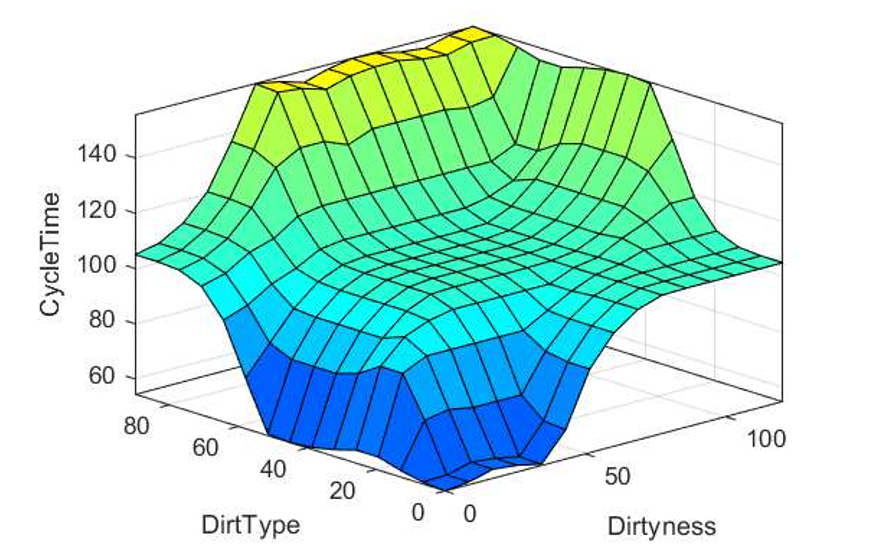
\includegraphics[width=.9\linewidth]{res/image1}
  \caption{Caption 1}
  \label{fig:sub1}
\end{subfigure}%
\begin{subfigure}{.5\textwidth}
  \centering
  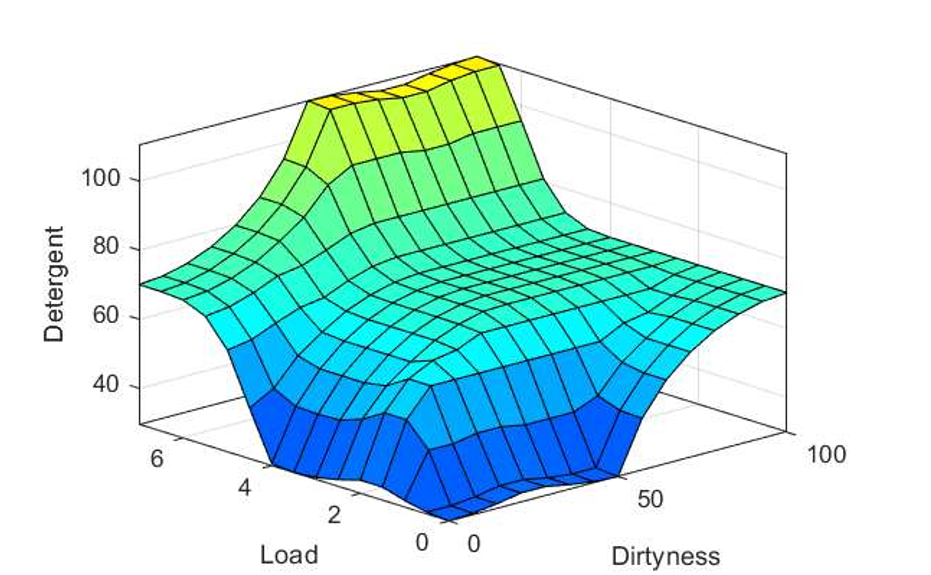
\includegraphics[width=.9\linewidth]{res/image2}
  \caption{Caption 2}
  \label{fig:sub2}
\end{subfigure}
\end{figure}

% Image
\begin{figure}[ht!]
\centering
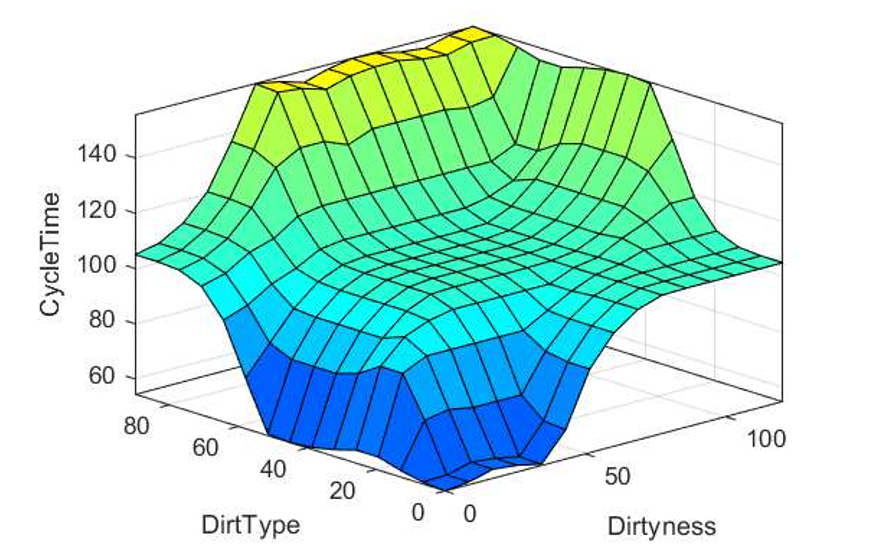
\includegraphics[width=.9\linewidth]{res/image1}
\caption{Caption 1}
\label{fig:sub1}
\end{figure}
